\documentclass[11pt]{article}
\usepackage{fullpage}
\usepackage{authblk}
\usepackage{graphicx}
 \usepackage{jabbrv}
\usepackage{amsmath}
\usepackage{amsfonts}
\usepackage{amssymb}
\usepackage{amsthm}
\usepackage{mathrsfs}
\usepackage{enumitem}
\usepackage{caption}
\usepackage{subcaption}
\captionsetup{compatibility=false} %This is to fix the issue that 'subcaption' package does not work correctly.

\newtheorem{theorem}{Theorem}%[section]
\newtheorem{lemma}[theorem]{Lemma}
\newtheorem{claim}[theorem]{Claim}
\newtheorem{corollary}[theorem]{Corollary}
\newtheorem{proposition}[theorem]{Proposition}
\newtheorem{definition}[theorem]{Definition}
\newtheorem{remark}[theorem]{Remark}
\newtheorem{assumption}[theorem]{Assumption}
\newtheorem{hypothesis}[theorem]{Hypothesis}
\newtheorem{observation}[theorem]{Observation}

\numberwithin{theorem}{section}

\makeatletter
\renewcommand\section{%
  \@startsection{section}{1}
                {\z@}%
                {-3.5ex \@plus -1ex \@minus -.2ex}%
                {2.3ex \@plus.2ex}%
                {\large\bfseries}% 11pt
}
\renewcommand\subsection{%
  \@startsection{subsection}{2}
                {\z@}%
                {-3.25ex\@plus -1ex \@minus -.2ex}%
                {1sp}% No space after subsections
                {\normalsize\bfseries}% normal size, boldface
}
\renewcommand\subsubsection{%
  \@startsection{subsubsection}{3}
                {\z@}%
                {-3.25ex\@plus -1ex \@minus -.2ex}%
                {1sp}% No space after subsubsections
                {\normalfont\normalsize}% normal size, medium
}
\makeatother

\marginparwidth 0pt \oddsidemargin 0pt \evensidemargin 0pt
\topmargin 30pt \textheight 21.0 truecm \textwidth 16.0 truecm

\title{{\Large\bf  On Kernel Mengerian Orientations of Line Graphs}}
\date{}
\author{Han Xiao \footnote{hxiao.math@connect.hku.hk}}

\affil{Department of Mathematics, 

The University of Hong Kong,

Hong Kong, China
}


\begin{document}

\numberwithin{equation}{section}

\maketitle
%\thispagestyle{empty}

\openup 1.2\jot

\hfill

\begin{abstract}
We present a polyhedral description of kernels in orientations of line graphs.
Given a digraph $D$, let $\sigma(D)$ denote the linear system consisting of domination, independence and nonnegativity constraints, and $FK(D)$ denote the set of all solutions to $\sigma(D)$. We call $D$ kernel ideal if $FK(D')$ is integral for each induced subgraph $D'$ of $D$ and kernel Mengerian if $\sigma(D')$ is TDI for each induced subgraph $D'$ of $D$. We also call $D$ good if it is clique-acyclic and each directed odd cycle has a chord.
We show that an orientation of a line graph is kernel ideal if and only if it is kernel Mengerian if and only if it is good. Our result strengthens the theorem of Borodin \textit{et al.} \cite{BoroKost98} on kernel perfect digraphs and generalizes the theorem of Kir\'{a}ly and Pap \cite{KiraPap08} on stable matching problem.

\hfill

\hfill

\noindent\textbf{AMS subject classifications:} 90C10, 90C27, 90C57.


\noindent\textbf{Key words:} kernel, stable matching, line graph, integral polytope, total dual integrality.
\end{abstract}


\newpage
\section{Introduction}
\label{intro}
An undirected graph is called \textit{simple} if it contains neither loops nor parallel edges and is called a \textit{multigraph} if parallel edges are allowed. 
\textit{Simple} digraphs and \textit{multidigraphs} are defined analogously. 

Let $G$ be an undirected graph.
The \textit{line graph} of $G$, denoted by $L(G)$, is an undirected graph that represents the adjacency of edges of $G$. 
We call $L(G)$ the \textit{line multigraph} of $G$ if any two vertices in $L(G)$ are joined by as many edges as the number of their common ends in $G$. 
Observe that there exist at most two parallel edges between any two vertices in a line multigraph.

Let $D=(V,A)$ be a digraph. 
For $U\subseteq V$, We call $U$ an \textit{independent} set of $D$ if no two vertices in $U$ are connected by an arc, call $U$ a \textit{dominating} set of $D$ if for each vertex $v\not\in U$, there is an arc from $v$ to $U$, and call $U$ a \textit{kernel} of $D$ if it is both independent and dominating. 
We call $D$ \textit{kernel perfect} if each of its induced subgraphs has a kernel.
A \textit{clique} of $D$ is a subset of $V$ such that every two distinct vertices are connected by an arc. We call $D$ \textit{clique-acyclic} if for every clique of $D$ the induced subdigraph of one-way arcs is acyclic, and call $D$ \textit{good} if it is clique-acyclic and each directed odd cycle has a chord or a pseudochord\footnote{A pseudochord is an arc $(v_i,v_{i-1})$ in a directed cycle $v_1 v_2\ldots v_l$}. 

\begin{theorem}[Borodin \textit{et al.} \cite{BoroKost98}]
\label{thm:BoroKost98}
Let $G$ be a line multigraph. The orientation $D$ of $G$ is kernel perfect if and only if it is good.
\end{theorem}

A subset $P$ of $\mathbb{R}^n$ is called a \textit{polytope} if it is the convex hull of finitely many vectors in $\mathbb{R}^n$. A point $x$ in $P$ is called a \textit{vertex} or an \textit{extreme point} if there exist no distinct points $y$ and $z$ in $P$ such that $x=\alpha y+ (1-\alpha)z$ for $0<\alpha<1$. It is well known that $P$ is the convex hull of its vertices, and that there exists a linear system $Ax\leq b$ such that $P=\{x\in\mathbb{R}^n:Ax\leq b\}$. Polytope $P$ is called $1/k$-\textit{integral} if its vertices are $1/k$-integral vectors, where $k\in\mathbb{N}$. By a theorem in linear programming, $P$ is $1/k$-integral if and only if $\max\{c^T x:Ax\leq b\}$ has an optimal $1/k$-integral solution for every integral vector $c$ for which the optimum is finite. If, instead, $\max\{c^T x:Ax\leq b\}$ has a dual optimal $1/k$-integral solution, we call linear system $Ax\leq b$ \textit{totally dual $1/k$-integral} (TDI$/k$).
It is easy to verify that $Ax\leq b$ is TDI$/k$ if and only if $Bx\leq b$ is TDI, where $B=A/k$ and $k\in\mathbb{N}$. Thus from a theorem of Edmonds and Giles \cite{EdmoGile77}, we deduce that if $Ax\leq b$ is TDI$/k$ and $b$ is integal, then $P=\{x\in\mathbb{R}^n:Ax\leq b\}$ is $1/k$-integral.

Let $\sigma(D)$ denote the linear system consisting of the following inequalities:
\begin{alignat}{4}
x(v)+x(N^+_{D}(v)) &\geq 1 &\qquad &\forall ~ v~&\in V, \label{domination constraints}\\
x(Q)&\leq 1 &\qquad &\forall ~ Q &\in \mathcal{Q}, \label{independence constraints}\\
x(v) &\geq 0 &\qquad &\forall ~ v~&\in V, \label{vertex nonnegativity}
\end{alignat}
where $x(U)=\sum_{u\in U}x(u)$ for any $U\subseteq V$, $N_D^+(v)$ denotes the set of all out-neighbors of vertex $v$, and $\mathcal{Q}$ denotes the set of all cliques of $D$. Observe that incidence vectors of kernels of $D$ are precisely integral solutions $x\in \mathbb{Z}^A$ to $\sigma(D)$.

The \textit{kernel polyotpe} of $D$, denoted by $K(D)$, is the convex hull of incidence vectors of all kernels of $D$.  The \textit{fractional kernel polytope} of $D$, denoted by $FK(D)$, is the set of all solutions $x\in \mathbb{R}^A$ to $\sigma(D)$. Clearly, $K(D)\subseteq FK(D)$.
We call $D$ \textit{kernel ideal} if $FK(D')$ is integral for each induced subgraph $D'$ of $D$, and \textit{kernel Mengerian} if $\sigma(D')$ is TDI for each induced subgraph $D'$ of $D$.

As described in Egres Open \cite{Egres}, the polyhedral description of kernels remains open. Chen \textit{et al.} \cite{ChenChen16} attained a polyhedral characterization of kernels by replacing clique constraints $x(Q)\leq 1$ for $Q\in\mathcal{Q}$ with independence constraints $x(u)+x(v)\leq 1$ for $(u,v)\in A$. In this paper we show that kernels in digraph $D$ can be thoroughly characterized by polyhedral approaches if $D$ is an orientation of line multigraphs.

\begin{theorem}
\label{thm:main}
Let $D$ be an orientation of a line multigraph. Then the following statements are equivalent:
\begin{enumerate}[label={\emph{(}\roman*\emph{)}}]
	\item $D$ is good;
	\item $D$ is kernel perfect;
	\item $D$ is kernel ideal;
	\item $D$ is kernel Mengerian.
\end{enumerate}
\end{theorem}

The equivalence of $(i)$ and $(ii)$ was established by Borodin \textit{et al.} \cite{BoroKost98} (Maffray \cite{Maff92} proved the case when the underlying undirected graph of $D$ is perfect). Kir\'{a}ly and Pap \cite{KiraPap08} proved the theorem when the underlying undirected graph of $D$ is the line graph of a bipartite graph, which will be given in the next section.
Our theorem strengthens the result of Borodin \textit{et al.} and generalizes the result of Kir\'{a}ly and Pap to line multigraphs.


\section{Preliminaries}
\label{pre}
Let $G=(V,E)$ be an undirected graph. For $v\in V$, let $\delta(v)$ be the set of all edges incident to $v$ and $\prec_v$ be a strict linear order on $\delta(v)$. We call $\prec_v$ the \emph{preference} of $v$ and say $v$ \emph{prefers} $e$ to $f$ or $e$ \emph{dominates} $f$ if $e\preceq_v f$ for $e,f\in \delta(v)$. Let $\prec$ be the set of all  $\prec_v$ for $v\in V$. We call $(G,\prec)$ a \emph{preference system} and call $(G,\prec)$ \emph{simple} if $G$ is simple. Let $M$ be a matching of $G$. We call $M$ \emph{stable} in $(G,\prec)$ if each edge of $G$ is dominated by some edge in $M$.

Let $(G,\prec)$ be a preference system. For $e\in E$, let $\varphi(e)$ denote the set of all edges of $G$ that dominate $e$. Let $\pi(G,\prec)$ be the linear system consisting of the following inequalites:
\begin{alignat}{3}
x(\varphi(e)) &\geq 1 &\qquad \forall ~e &\in E,\label{stability constraints}\\
x(\delta(v)) &\leq 1 &\qquad \forall ~v &\in V,\label{matching constraints}\\
x(e) &\geq 0 &\qquad \forall ~e &\in E.\label{edge nonnegativity}
\end{alignat}
As observed by Abeledo and Rothblum \cite{AbelRoth94}, incidence vectors of stable matchings of $(G,\prec)$ are precisely integral solutions $x\in \mathbb{Z}^E$ to $\pi(G,\prec)$.

The \textit{stable matching polytope}, denoted by $SM(G,\prec)$, is the convex hull of incidence vectors of all stable matchings of $(G,\prec)$. The \textit{fractional stable matching polytope}, denoted by $FSM(G,\prec)$, is the set of all solutions $x\in \mathbb{R}^E$ to $\pi(G,\prec)$. Clearly, $SM(G,\prec)\subseteq FSM(G,\prec)$. 

\begin{theorem}[Rothblum \cite{Roth92}]
\label{thm:Roth92}
Let $(G,\prec)$ be a simple preference system. If $G$ is bipartite, then
$SM(G,\prec)=FSM(G,\prec)$.
\end{theorem}

\begin{theorem}[Kir\'{a}ly and Pap \cite{KiraPap08}]
\label{thm:KiraPap08}
Let $(G,\prec)$ be a simple preference system. If $G$ is bipartite, then $\pi(G,\prec)$ is totally dual integral.
\end{theorem}

Let $C=v_1 v_2 \ldots v_l$ be a cycle in $G$, we say that $C$ has \textit{cyclic preferences} in $(G,\prec)$ if
$v_{i-1} v_i \prec_{v_i} v_i v_{i+1}$ for $i=1,2,\ldots,l$
or $v_{i-1} v_i\succ_{v_i} v_i v_{i+1}$ for $i=1,2,\ldots,l$,
where indices are taken modulo $l$.
For $x\in FSM(G,\prec)$, let $E_{\alpha}(x)$ denote the set of all edges with $x(e)=\alpha$ where $\alpha\in\mathbb{R}$ and $E_+(x)$ denote the set of all edges with $x(e)>0$.

\begin{theorem}[Abeledo and Rothblum \cite{AbelRoth94}]
\label{thm:AbelRoth94}
Let $(G,\prec)$ be a simple preference system. Then $FSM(G,\prec)$ is $1/2$-integral. Moreover, for each $1/2$-integral point $x$ in $FSM(G,\prec)$, $E_{1/2}(x)$ consists of vertex disjoint cycles with cyclic preferences.
\end{theorem} 

\begin{theorem}[Chen \textit{et al.} \cite{ChenDing12}]
\label{thm:ChenDing12}
Let $(G,\prec)$ be a simple preference system. Then $\pi(G,\prec)$ is totally dual $1/2$-integral. Moreover, $\pi(G,\prec)$ is totally dual integral if and only if $SM(G,\prec)=FSM(G,\prec)$.
\end{theorem}

\section{Reductions}
To study kernels in multidigraphs, it suffices to work on its minimal spanning subdigraph that  preserves all the connection relations of vertices. In the remainder of this paper, we assume that $D$ is an orientation of line multigraph $L(H)$ such that any two vertices in $H$ are joined by at most two edges and parallel edges in $L(H)$ are orientated oppositely. Hence $D$ is a multidigraph such that any two distinct vertices are joined by at most one arc in each direction.

Kernels are closely related to stable matchings. Let $D$ be a clique-acyclic orientation of line multigraph $L(H)$. 
For any two adjacent edges $e$ and $f$ in $H$, define $e\prec_v f$ if $(e,f)$ is an arc in $D$, where $v$ is a common end of $e$ and $f$.
Hence each clique-acyclic orientation $D$ of line multigraph $L(H)$ is associated with a preference system $(H,\prec)$.
Recall that $\sigma(D)$ denotes the linear system which defines $FK(D)$. 
Consequently, $\sigma(D)$ can be viewed as a linear system defined on preference system $(H,\prec)$. 
The equivalence of constraints (\ref{vertex nonnegativity}) and constraints (\ref{edge nonnegativity}) follows directly. Constraints (\ref{domination constraints}) can be viewed as constraints (\ref{stability constraints}) because of the one to one correspondence between dominating vertex set $\{v\}\cup N^+_D(v)$ for $v\in V(D)$ and stable edge set $\varphi(e)$ for $e\in E(H)$.
Observe that cliques of $D$ correspond to three types of edge sets in $H$:
\begin{itemize}
\item $\delta(v)$ for $v\in V(H)$,
\item nontrivial subsets of $\delta(v)$ for $v\in V(H)$,
\item complete subgraphs of $H$ induced on three vertices (with parallel edges allowed).
\end{itemize}
Hence constraints (\ref{independence constraints}) can be viewed as constraints (\ref{matching constraints}) together with some extra constraints on $(H,\prec)$. Let $\mathcal{O}(H)$ denote the set of all complete subgraphs of $H$ induced on three vertices. 
Then $\sigma(D)$ can be reformulated in terms of preference system $(H,\prec)$:
\begin{alignat}{4}
x(\varphi(e)) &\geq 1 &\qquad &\forall ~e &\in E(H),\label{constraints:1}\\
x(\delta(v)) &\leq 1 &\qquad &\forall ~v &\in V(H),\label{constraints:2}\\
x(S) &\leq 1 &\qquad \emptyset\subset S\subset \delta(v),\quad &\forall ~v&\in V(H),\label{constraints:3}\\
x(O) &\leq 1 &\qquad &\forall ~O&\in \mathcal{O}(H),\label{constraints:4}\\
x(e) &\geq 0 &\qquad &\forall ~e &\in E(H)\label{constraints:5}.
\end{alignat}
Notice that constraints (\ref{constraints:1}), (\ref{constraints:2}) and (\ref{constraints:5}) constitute the Rothblum system $\pi(H,\prec)$ which defines $FSM(H,\prec)$. Constraints (\ref{constraints:3}) are redundant with respect to $\pi(H,\prec)$ due to constraints (\ref{constraints:2}). As we shall see, constraints (\ref{constraints:4}) are also redundant with respect to $\pi(H,\prec)$ when $D$ is good. Hence $FK(D)$ is essentially defined by Rothblum system $\pi(H,\prec)$, or equivalently, that $FK(D)=FSM(H,\prec)$, when $D$ is good.

\begin{lemma}
\label{lem:reduct1}
For parallel edges $e$ and $e'$ in $H$, there exists no edge $f$ such that $e\prec_v f \prec_v e'$, where $v$ is a common end of $e$ and $e'$.
\end{lemma}
\begin{proof}
Since $D$ is clique-acyclic, by the construction of preference system $(H,\prec)$, the lemma follows directly.
\end{proof}

By Lemma \ref{lem:reduct1}, parallel edges play exactly the same role in preference system $(H,\prec)$. Hence we turn to study underlying simple preference systems of $(H,\prec)$. Let $(\hat{H},\hat\prec)$ be a simple preference system, where $\hat{H}$ is a spanning subgraph of $H$ obtained by keeping one edge between every pair of adjacent vertices and $\hat\prec$ is the restriction of $\prec$ on $\hat{H}$. Before proceeding, we introduce a technical lemma first.

\begin{lemma}
\label{lem:reduct2}
Let 
\begin{equation}\label{equ:syst.}
Ax\leq b,~x\geq 0
\end{equation}
and
\begin{equation}\label{equ:syst. with duplicate columns}
\bar{A}\bar{x}\leq b,~\bar{x}\geq 0
\end{equation}
be two linear systems, where $\bar{A}$ is obtained from $A$ by duplicating some columns. If (\ref{equ:syst.}) is totally dual $1/k$-integral, then so is (\ref{equ:syst. with duplicate columns}), where $k\in \mathbb{N}$.
\end{lemma}
\begin{proof}
It suffices to prove that the theorem holds for $\bar{A}$ with one duplicate column.
Let $\bar{x}:=(\bar{x}_1,\ldots,\bar{x}_{n+1})\in\mathbb{R}^{n+1}$ and $\bar{A}:=(\bar{a}_1,\ldots,\bar{a}_{n+1})=(A,a_{k})$, where $a_k$ is the $k$th column of $A$. Let $\bar{c}:=(\bar{c}_1,\ldots,\bar{c}_{n+1})\in \mathbb{Z}^{n+1}$ be an arbitrary integral vector such that $\max\{\bar{c}^T \bar{x}: \bar{A}\bar{x}\leq b,~\bar{x}\geq 0\}$ is finite. 

Let $\hat{c}\in \mathbb{Z}^n$ be defined by
\begin{equation*}
\hat{c}_i:=
\begin{cases}
\bar{c}_i & i\not=k,\\
\max\{\bar{c}_k, \bar{c}_{n+1}\} & i=k,
\end{cases}
\end{equation*}
and $\hat{x}\in \mathbb{R}^n$ be defined by
\begin{equation*}
\hat{x}_i:=
\begin{cases}
\bar{x}_i & i\not=k,\\
\bar{x}_k+\bar{x}_{n+1} & i=k.
\end{cases}
\end{equation*}
Clearly,  $\max\{\hat{c}^T \hat{x}:A\hat{x}\leq b,~\hat{x}\geq 0\}\geq\max\{\bar{c}^T \bar{x}:\bar{A}\bar{x}\leq b,~\bar{x}\geq 0\}$. We claim that equality always holds in this inequality. Given an arbitrary optimal solution $\hat{x}^*$ to $\max\{\hat{c}^T \hat{x}:A\hat{x}\leq b,~\hat{x}\geq 0\}$, define $\bar{x}^*$ by $\bar{x}^*_i:=\hat{x}^*_i$ for $i\not=k,n+1$, if $\bar{c}_k>\bar{c}_{n+1}$, $\bar{x}^*_k:=\hat{x}^*_k$ and $\bar{x}^*_{n+1}:=0$, otherwise $\bar{x}^*_k:=0$ and $\bar{x}^*_{n+1}:=\hat{x}^*_k$. It is easy to verify that $\bar{x}^*$ is a feasible solution to $\max\{\bar{c}^T \bar{x}:\bar{A}\bar{x}\leq b,~\bar{x}\geq 0\}$. Moreover, $\hat{c}^T\hat{x}^*=\bar{c}^T\bar{x}^*$ implies $\max\{\hat{c}^T \hat{x}:A\hat{x}\leq b,~\hat{x}\geq 0\}\leq\max\{\bar{c}^T \bar{x}:\bar{A}\bar{x}\leq b,~\bar{x}\geq 0\}$. Hence equality follows.

Since $Ax\leq b$ is TDI$/k$, there exists a dual optimal $1/k$-integral solution $y^*$ to $\max\{\hat{c}^T\hat{x}:A\hat{x}\leq b,~\hat{x}\geq 0\}$ such that $(y^*)^T b=\max\{\hat{c}^T \hat{x}:A\hat{x}\leq b,~\hat{x}\geq 0\}$, $(y^*)^T A\geq \hat{c}^T$ and $y^*\geq 0$. It follows that
\begin{equation*}
(y^*)^T \bar{A}=(y^*)^T (A,a_k)=((y^*)^T A,(y^*)^T a_k)\geq (\hat{c}^T,\hat{c}_k)\geq\bar{c}^T,
\end{equation*}
implying that $y^*$ is a feasible dual solution to $\max\{\bar{c}^T \bar{x}:\bar{A}\bar{x}\leq b,~\bar{x}\geq 0\}$. By the following inequalities
\begin{equation*}
(y^*)^T b=\max\{\hat{c}^T \hat{x}:A\hat{x}\leq b,~\hat{x}\geq 0\}=\max\{\bar{c}^T \bar{x}:\bar{A}\bar{x}\leq b,~\bar{x}\geq 0\}\leq (y^*)^T b,
\end{equation*} $y^*$ is also a dual optimal solution to $\max\{\bar{c}^T \bar{x}:\bar{A}\bar{x}\leq b,~\bar{x}\geq 0\}$, where the last inequality is from the weak duality theorem. Hence the lemma follows.
\end{proof}

\begin{lemma}
\label{lem:reduct3}
If $\pi(\hat{H},\hat\prec)$ is totally dual $1/k$-integral, then so is $\pi(H,\prec)$, where $k\in\mathbb{N}$.
\end{lemma}
\begin{proof}
By Lemma \ref{lem:reduct1}, columns corresponding to parallel edges in the left hand side matrix of $\pi(H,\prec)$ are identical. Hence the left hand side matrix of $\pi(H,\prec)$ can be obtained from that of $\pi(\hat{H},\hat\prec)$ by duplicating columns corresponding to parallels edges. Then the lemma follows from Lemma \ref{lem:reduct2}.
\end{proof}

By Theorem \ref{thm:ChenDing12} and Lemma \ref{lem:reduct3}, we conclude that $\pi(H,\prec)$ is TDI$/2$. By the construction of $(H,\prec)$, when $D$ is good $(H,\prec)$ admits no odd cycles with cyclic preferences. It follows that constraints (\ref{constraints:4}) are redundant with respect to $\pi(H,\prec)$ when $D$ is good.

\begin{lemma}
\label{lem:reduct4}
$FSM(H,\prec)$ is integral if and only if $FSM(\hat{H},\hat\prec)$ is integral.
\end{lemma}
\begin{proof}
For simplicity, assume that $H=(V,E)$ and $\hat{H}=(V,\hat{E})$.

We prove the only if part by showing that $FSM(\hat{H},\hat\prec)$ is a projection of $FSM(H,\prec)$. 
Let $\hat{x}$ be a point in $FSM(\hat{H},\hat\prec)$ and define $x:=(\hat{x},0)\in \mathbb{R}^{\hat{E}}\times \mathbb{R}^{E-\hat{E}}$. To show that $x\in FSM(H,\prec)$, it suffices to prove that $x(\varphi(e))\geq 1$ for $e\in E-\hat{E}$. Let $e'\in \hat{E}$ be the edge parallel with $e\in E-\hat{E}$. By Lemma \ref{lem:reduct1}, $x(\varphi(e))=x(\varphi(e'))=\hat{x}(\varphi(e'))\geq 1$. Hence $FSM(\hat{H},\hat\prec)$ is a projection of $FSM(H,\prec)$.

We prove the if part by showing that each vertex of $FSM(H,\prec)$ can be obtained from some vertex of $FSM(\hat{H},\hat\prec)$ by adding some zero entries. Let $x$ be a vertex of $FSM(H,\prec)$. Define $\hat{x}\in \mathbb{R}^{\hat{E}}$ by, for $e\in \hat{E}$, $\hat{x}(e):=x(e)+x(e')$, where $e'\in E-\hat{E}$ is parallel with $e$. By Lemma \ref{lem:reduct1}, it is easy to verify that $\hat{x}\in FSM(\hat{H},\hat\prec)$. We claim that $\hat{x}$ is a vertex of $FSM(\hat{H},\hat\prec)$. Assume to the contrary that there exist $\hat{x}_1, \hat{x}_2 \in FSM(\hat{H},\hat\prec)$ such that $\hat{x}=\alpha \hat{x}_1+ (1-\alpha)\hat{x}_2$, where $0<\alpha<1$. For $i=1,2$, we extend $\hat{x}_i\in \mathbb{R}^{\hat{E}}$ to $x_i\in \mathbb{R}^{E}$ by, for $e\in \hat{E}$ without parallel edges in $H$, $x_i(e):=\hat{x}_i(e)$; for $e\in\hat{E}$ and its parallel edge $e'\in E-\hat{E}$, if $x(e)>x(e')$, $x_i(e):=\hat{x}_i(e)$ and $x_i(e'):=0$, otherwise $x_i(e):=0$ and $x_i(e'):=\hat{x}_i(e)$. By Lemma \ref{lem:reduct1}, it is easy to see that $x_1,x_2\in FSM(H,\prec)$. Furthermore, $x(e)\cdot x(e')=0$ for parallel edges $e$ and $e'$. Assume to the contrary that $x(e)\cdot x(e')\not=0$, then $x(e)=x(e')=1/2$. Let $y$ and $z$ be duplicates of $x$ and set $y (e):=z(e'):=1$ and $y (e'):=z(e):=0$. It follows that $x= (y + z)/2$. Clearly, $y,z\in FSM(H,\prec)$, contradicting to the assumption that $x$ is a vertex.
Now since $x(e)\cdot x(e')=0$ for parallel edges $e$ and $e'$, $x=\alpha x_1+(1-\alpha) x_2$ follows, a contradiction. Hence $\hat{x}$ is vertex of $FSM(\hat{H},\hat\prec)$. Therefore each vertex $x$ of $FSM(H,\prec)$ is associated with a vertex $\hat{x}$ of $FSM(\hat{H},\hat\prec)$ and $x$ can be obtained from $\hat{x}$ by, for $e\in \hat{E}$ without parallel edges in $H$, $x(e):=\hat{x}(e)$; for $e\in\hat{E}$ and its parallel edge $e'\in E-\hat{E}$, if $x(e)>x(e')$, $x(e):=\hat{x}(e)$ and $x(e'):=0$, otherwise $x(e):=0$ and $x(e'):=\hat{x}(e)$. 
\end{proof}

We end this section with a summary. Let $D$ be an orientation of line multigraph $L(H)$. When $D$ is clique-acyclic, it is associated with a preference system $(H,\prec)$ and a simple preference system $(\hat{H},\hat\prec)$, where $\hat{H}$ is a simple spanning subgraph of $H$ maximizing the edge set and $\hat\prec$ is the restriction of $\prec$ on $\hat{H}$.
Hence constraints (\ref{constraints:3}) and (\ref{constraints:4}) are redundant in $\sigma(D)$ with respect to $\pi(H,\prec)$ and $FK(D)=FSM(H,\prec)$. To show $FK(D)$ is integral, by Lemma \ref{lem:reduct4} it suffices to show that $FSM(\hat{H},\hat\prec)$ is integral. To show $\sigma(D)$ is TDI, by Lemma \ref{lem:reduct3} it suffices to show $\pi(\hat{H},\hat\prec)$ is TDI. Moreover, when $D$ is good both $(H,\prec)$ and $(\hat{H},\hat\prec)$ admit no odd cycles with cyclic preferences.

\section{Proofs}
Before presenting our proof to the main theorem, we explore some properties of simple preference systems admitting no odd cycles with cyclic preferences.
\begin{lemma}
\label{lem:prf1}
Let $(G,\prec)$ be a simple preference system. If $(G,\prec)$ admits no odd cycles with cyclic preferences, then $SM(G,\prec)=FSM(G,\prec)$.
\end{lemma}

As observed by Chen \textit{et al.} \cite{ChenDing12}, integrality of $FSM(G,\prec)$ is equivalent to total dual integrality of $\pi(G,\prec)$, where $(G,\prec)$ is a simple preference system. A corollary follows directly.

\begin{corollary}
\label{cor:prf2}
Let $(G,\prec)$ be a simple preference system. If $(G,\prec)$ admits no odd cycles with cyclic preferences, then $\pi(G,\prec)$ is totally dual integral.
\end{corollary}

\begin{proof}[Proof of Lemma \ref{lem:prf1}]
Let $(G,\prec)$ be a simple preference system admitting no odd cycles with cyclic preferences.
By Theorem \ref{thm:AbelRoth94}, $FSM(G,\prec)$ is $1/2$-integral.
Let $x$ be a $1/2$-integral point in $FSM(G, \prec)$.
Consider $E_{1/2}(x)$, which consists of even cycles $C_1,C_2,\ldots,C_r$ with cyclic preferences. For $i=1,2,\ldots,r$, label vertices and edges of $C_i\in E_{1/2}(x)$ such that $C_i=v^i_1v^i_2\ldots v^i_{l}$ and $e^i_k\prec_{v^i_{k+1}} e^i_{k+1}$ for $k=1,2,\ldots,l$, where $e^i_k=v^i_{k}v^i_{k+1}$ and indices are taken modulo $l$. 
We remark that the parity of vertices and edges refers to the parity of their indices. Define $z\in \mathbb{R}^{E(G)}$ by
\begin{equation*}
z(e):=
\begin{cases}
1 & e\text{ is an even edge in some }C \in E_{1/2}(x),\\
-1 & e\text{ is an odd edge in some }C \in E_{1/2}(x),\\
0 & \text{otherwise}.
\end{cases}
\end{equation*}
We are going to exclude $x$ from vertices of $FSM(G, \prec)$ by adding perturbation $\epsilon z$ for small $\epsilon$ to $x$ and showing that $x\pm\epsilon z\in FSM(G,\prec)$. 
Tight constraints in (\ref{stability constraints})-(\ref{edge nonnegativity}) under perturbation $\epsilon z$ play a key role here. Observe that tight constraints in (\ref{matching constraints}) and (\ref{edge nonnegativity}) are invariant under perturbation $\epsilon z$. It remains to show that perturbation $\epsilon z$ does not affect tight constraints in (\ref{stability constraints}) either. Let $e$ be an edge with $x(\varphi(e))=1$. Clearly, $\lvert \varphi(e)\cap E_+(x)\rvert \in\{1,2\}$. When $\lvert \varphi(e)\cap E_+(x)\rvert=1$, $x(e)=1$ follows, which is trivial. When $\lvert \varphi(e)\cap E_+(x)\rvert =2$, we claim that the parity of dominating edges in $E_{1/2}(x)$ of $e$ does not agree (relabeling vertices and edges in $E_{1/2}(x)$ if necessary).
Hence corresponding tight constraints in (\ref{stability constraints}) are also invariant under perturbation $\epsilon z$.

To justify this claim, we distinguish four cases.

\textbf{Case 1.} Edge $e$ is an edge from some $C\in E_{1/2}(x)$. This case is trivial since $C$ admits cyclic preferences.

\textbf{Case 2.} Edge $e$ is a chord in some $C\in E_{1/2}(x)$. We first show that endpoints of $e$ have different parity in $C$. We prove it by contradiction. Without loss of generality, let $e=v_{2i}v_{2j}$.
\begin{figure}
\centering
\begin{subfigure}{.4\textwidth}
  \centering
  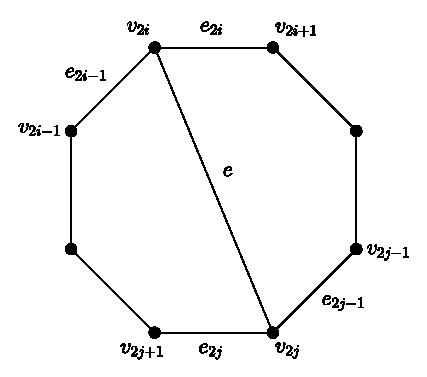
\includegraphics[width=.85\linewidth]{KernelMengerianO-fig1a}
  \caption{}
  \label{fig1a}
\end{subfigure}%
\begin{subfigure}{.4\textwidth}
  \centering
  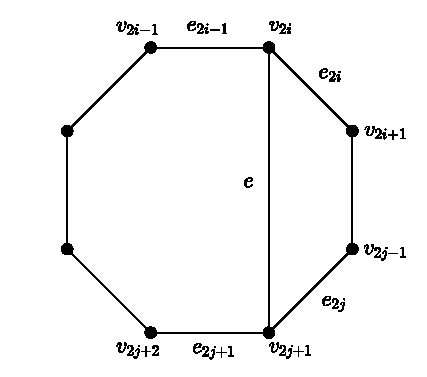
\includegraphics[width=.845\linewidth]{KernelMengerianO-fig1b}
  \caption{}
  \label{fig1b}
\end{subfigure}
\caption{Case 2}
\end{figure}
If $e_{2i}\prec e$, then $e_{2i-1}\prec e$. By assumption $x(\varphi(e))=1$, it follows that $e\prec e_{2j-1}$ and $e\prec e_{2j}$. However, $v_{2i} e v_{2j} e_{2j} v_{2j+1} \ldots v_{2i-1} e_{2i-1} v_{2i}$ consistute an odd cycle with cyclic preferences, a contradiction. Hence $e\prec e_{2i}$.

Similarly, if $e_{2j}\prec e$, then $e_{2j-1}\prec e$. Eqaulity $x(\varphi(e))=1$ implies that $e\prec e_{2i}$ and $e\prec e_{2i-1}$. However, $v_{2i} e_{2i} v_{2i+1} \ldots v_{2j-1} e_{2j-1} v_{2j} e v_{2i}$ constitute an odd cycle with cyclic preferences, a contradiction. Hence $e\prec e_{2j}$. 

Now $e\prec e_{2i}$ and $e\prec e_{2j}$, it follows that $e_{2i-1}\prec e$ and $e_{2j-1}\prec e$ since $x(\varphi(e))=1$. But in this case two odd cycles with cyclic preferences mentioned above occur at the same time. 
Therefore, endpoints of $e$ have different parity in $C$. Let $e=v_{2i} v_{2j+1}$.
If $e_{2i}\prec e$ (\textit{resp.} $e_{2j+1}\prec e$), it follows that $e_{2i-1}\prec e$ (\textit{resp.} $e_{2j}\prec e$). Then $e$ is dominated by two consecutive edges from $C$, which is trivial.  So assume that $e\prec e_{2i}$ and $e\prec e_{2j+1}$. Since $x(\varphi(e))=1$, it follows that $e_{2i+1}\prec e$ and $e_{2j}\prec e$. Hence e is dominated by two edges with different parity.

\textbf{Case 3.} Edge $e$ is a hanging edge of some $C\in E_{1/2}(x)$ and dominated by two edges from $C$. This case is trivial.

\textbf{Case 4.} Edge $e$ is a connecting edge bewteen $C_i$ and $C_j$ and dominated by one edge from $C_i$ and one edge from $C_j$ respectively, where $C_i, C_j \in E_{1/2}(x)$.
For $k=1,2,\ldots,r$, let $F_k$ be a subset of edges in case 4 incident to $C_k$.
\begin{figure}
\centering
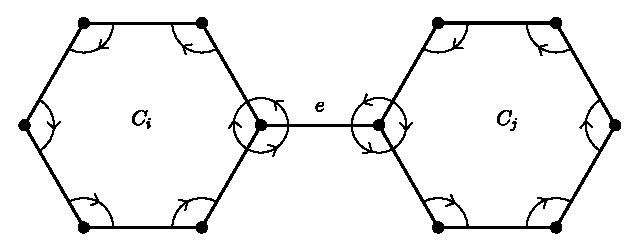
\includegraphics[scale=0.85]{KernelMengerianO-fig2}
\caption{Case 4}
\end{figure}
Then $\cup_{i=1}^{i=r} F_i\cup C_i$ induces a subgraph of $G$. It suffices to work on a component of the induced subgraph. We apply induction on the number $\alpha$ of cycles from $E_{1/2}(x)$ in a component.

When $\alpha=1$, it is trivial.
Hence assume the claim holds for components with $\alpha\geq 1$ cycles from $E_{1/2}(x)$. We consider a component with $\alpha +1$ cycles $C_1, \ldots, C_{\alpha}, C_{\alpha+1}$ from $E_{1/2}(x)$. 
Without loss of generality, assume that deleting $C_{\alpha+1}$ yields a new component with $\alpha$ cycles.
By induction hypothesis, the claim holds for the resulting component. 
It remains to check edges in $F_{\alpha+1}$. If there exists an edge in $F_{\alpha+1}$ violating the claim, we relabel vertices and edges in $C_{\alpha+1}$. After at most one relabeling, all edges in $F_{\alpha+1}$ satisfy the claim. We prove it by contradiction. Let $f_1,f_2 \in F_{\alpha +1}$ be edges such that $f_1$ satisfies the claim but $f_2$ violates the claim. For $i=1,2$, let $f_i=u_i w_i$, where $u_i$ is the endpoint in the resulting component and $w_i$ is the endpoint in $C_{\alpha+1}$. By assumption, $u_1$ and $w_1$ have different parity and $u_2$ and $w_2$ have the same parity.
Analogous to the definition of cycles with cyclic preferences, we call path $P=v_1 v_2 \ldots v_l$ a \textit{$v_1 v_l$-path with linear preferences} if $v_iv_{i+1}\prec_{v_{i+1}}v_{i+1}v_{i+2}$ for $i=1,2,\ldots,l-2$. Clearly, for any two vertices in the same component, there exists a path with linear preferences between them.
Hence there exists a $u_1 u_2$-path $P_\alpha$ and a $w_2 w_1$-path $P_{\alpha+1}$, both of which admit linear preferences.
Moreover, $u_1 P_\alpha u_2 f_2 w_2 P_{\alpha+1} w_1 f_1 u_1$ constitute a cycle with cyclic preferences. We justify this cycle is odd by 
showing that the $u_1 u_2$-path $P_\alpha$ is even (\textit{resp.} odd) if $u_1$ and $u_2$ have the same (\textit{resp.} different) parity.

If $u_1$ and $u_2$ are from the same cycle $C_k$, where $k\in \{1,2,\ldots,\alpha\}$, it is trivial. Hence assume $u_1=v^s \in C_s$ and $u_2=v^t\in C_t$, where $s,t\in \{1,2,\ldots,\alpha\}$ and $s\not=t$. We apply induction on the number $\tau$ of cycles from $E_{1/2}(x)$ involved in $P_\alpha$. Clearly, $\tau\geq 2$.
When $\tau=2$. Take $v^s_+ v^t_-\in F_s\cap F_t$ on $P_\alpha$. Let $P_s$ be the part of $P_\alpha$ from $v^s$ to $v^s_+$ in $C_s$ and $P_t$ be the part of $P_\alpha$ from $v^t_-$ to $v^t$ in $C_t$. It follows that $v^sP_s v^s_+ v^t_- P_t v^t$ constitute $P_\alpha$. By assumption, $v^s_+$ and $v^t_-$ have different parity since $v^s_+ v^t_-\in F_s\cap F_t$. If $v^s$ and $v^t$ have the same parity, then $P_s$ and $P_t$ have different parity, implying that $P_\alpha$ is even; if $v^s$ and $v^t$ have different parity, then $P_s$ and $P_t$ have the same parity, implying that $P_\alpha$ is odd.
Now assume $\tau\geq 2$. Let $C_{k_1},\ldots,C_{k_\tau},C_{k_{\tau+1}}$ be cycles from $E_{1/2}(x)$ involved along $P_\alpha$. Take $v^{k_{\tau}}_+ v^{k_{\tau+1}}_- \in F_{k_{\tau}}\cap F_{k_{\tau+1}}$ on $P_\alpha$. Let $P_{s, k_{\tau}}$ denote the part of $P_\alpha$ from $v^s$ to $v^{k_{\tau}}_+$ and $P_{k_{\tau},t}$ denote the part of $P_\alpha$ from $v^{k_{\tau}}_+$ to $v^t$. Clearly, $P_\alpha=v^sP_{s,k_\tau} v^{k_\tau}_+ P_{k_\tau, t} v^t$. Since $P_{s, k_{\tau}}$ involves $\tau$ cycles and $P_{k_{\tau},t}$ involves two cycles, the length of both depends on the parity of endpoints. It follows that $P_\alpha$ is even when $u_1$ and $u_2$ have the same parity and $P_\alpha$ is odd when $u_1$ and $u_2$ have different parity.

By assumption, when $u_1$ and $u_2$ have the same parity, $w_1$ and $w_2$ have different parity, implying that $P_\alpha$ is even and $P_{\alpha+1}$ is odd;
when $u_1$ and $u_2$ have different parity, $w_1$ and $w_2$ have the same parity, implying that $P_\alpha$ is odd and $P_{\alpha+1}$ is even. 
Either case yields an odd cycle with cyclic preferences, a contradiction.

Therefore $1/2$-integral points are not vertices of $FSM(G,\prec)$ as they can be perturbed by $\epsilon z$ for small $\epsilon$ without leaving $FSM(G,\prec)$ . By Theorem \ref{thm:AbelRoth94}, $SM(G,\prec)=FSM(G,\prec)$ follows. 
\end{proof}

Now we are ready to present a proof to our main theorem.

\begin{proof}[Proof of Theorem \ref{thm:main}]
It suffices to show the equivalence of $(i)$, $(iii)$ and $(iv)$. Without loss of generality, let $D$ be an orientation of line multigraph $L(H)$ such that any two vertices in $H$ are joined by at most two edges and parallel edges in $L(H)$ are orientated oppositely. When $D$ is good, $D$ is associated with a preference system $(H,\prec)$ and a simple preference system $(\hat{H},\hat\prec)$, both of which admit no odd cycles with cyclic preferences, where $\hat{H}$ is a simple spanning subgraph of $H$ maximizing the edge set and $\hat\prec$ is the restriction of $\prec$ on $\hat{H}$.
Hence $\sigma(D)$ can be viewed as a linear system defined on preference system $(H,\prec)$ and consisting of constraints (\ref{constraints:1})-(\ref{constraints:5}), where constraints (\ref{constraints:1}), (\ref{constraints:2}) and $(\ref{constraints:5})$ constitute the Rothblum system $\pi(H,\prec)$.

By Lemma \ref{lem:prf1}, $FSM(\hat{H},\hat\prec)$ is integral. Integrality of $FSM(H,\prec)$ follows from Lemma \ref{lem:reduct4}. Hence constraints (\ref{constraints:3}) and (\ref{constraints:4}) are both redundant in $\sigma(D)$ with respect to $\pi(H,\prec)$. Therefore $FK(D)=FSM(H,\prec)$, implying that $FK(D)$ is integral. Similar arguments apply to any induced subgraphs of $D$. Hence $(i)\implies (iii)$. 

By Corollary \ref{cor:prf2}, $\pi(\hat{H},\hat\prec)$ is TDI. Total dual integrality of $\pi(H,\prec)$ follows from Lemma \ref{lem:reduct3}. Since $\pi(H,\prec)$ is part of $\sigma(D)$ and the other constraints (\ref{constraints:3})-(\ref{constraints:4}) are redundant in $\sigma(D)$ with respect to $\pi(H,\prec)$, total dual integrality of $\sigma(D)$ follows. Similar arguments apply to any induced subgraphs of $D$. Hence $(iii)\implies (iv)$.

By a theorem of Edmonds and Giles \cite{EdmoGile77}, $(iv)\implies (iii)$ follows directly.

To see $(iii)\implies (i)$, we prove it by contradiction. Observe that strong kernel idealness of  $D$ implies the existence of kernels for any induced subgraphs of $D$. Let $D$ be a digraph such that D is kernel ideal but not good. Then there exists either a clique containing directed cycles or a directed odd cycle without chords nor pseudochords in $D$. We show that neither case is possible. If $D$ has a clique containing directed cycles, we consider the subgraph induced on this clique. There is no kernel for this induced subgraph, a contradiction. If $D$ contains a directed odd cycle without chords nor pseudochords, we restrict ourselves to the subgraph induced on this directed odd cycle. There is no kernel for this induced subgraph either, a contradiction.
\end{proof}

\section*{Acknowledgments}
The author would like to thank Prof. Wenan Zang for his invaluable suggestions.

\bibliographystyle{jabbrv_siam}
\bibliography{KernelMengerianO}
\nocite{Schr86}

\end{document}
